\documentclass[12pt,oneside,a4paper]{article}

%% Language and font encodings
\usepackage{textcomp}
\usepackage{ulem}
\usepackage[danish,english]{babel}
\usepackage[utf8x]{inputenc}
\usepackage[T1]{fontenc}

%% Sets page size and margins
\usepackage[left=2.5cm,top=2.0cm,bottom=1.5cm, right=3.0cm]{geometry}

%% Useful packages
\usepackage{amsmath}
\usepackage{graphicx}
\usepackage{epsfig}
\usepackage[colorinlistoftodos]{todonotes}
\usepackage[colorlinks=true, allcolors=blue]{hyperref}
\usepackage{gensymb}
\usepackage{float}
\usepackage{adjustbox}
\usepackage{graphics}
\usepackage{amssymb}
\usepackage{url}
\usepackage{cancel}
\usepackage{booktabs}
\usepackage{pdfpages}
\usepackage{mathpazo}
\usepackage[section]{placeins}
\usepackage{caption}
\usepackage{wrapfig}
\usepackage{tocloft}
\usepackage{subfig}
\usepackage{fancyhdr}
\usepackage{framed}
\usepackage{footnote}

\linespread{1.3} % linjeafstand 1.5
\setlength{\parindent}{0cm}
\setlength{\parskip}{0.3cm}

\begin{document}
\selectlanguage{danish}
\pagenumbering{roman}

%% Forside %%

\begin{center}
    {\textsc {\LARGE \bf{Københavns Universitet \\[0.3cm]  Bachelorstudiet i fysik}}}\\[1.5cm]
    {\textsc {\Large \bf Førsteårsprojekt 2017}}\\[0.8cm]
    {\Large Projekt nummer: 2017-05}\\[1cm]
    
    \rule{15cm}{0.01cm}\\[1cm]
    {\LARGE\bf  Simulering af neutron optik} \\ {\it Med fokus på M-Optimization}\\ [0.5cm]
    \rule{15cm}{0.01cm}\\[1cm]
\end{center}

\vfill
{\large Forfattere:}\\
{\large \hspace*{1cm} \makebox[6cm][l]{Jonas Peter Hyatt}  \hspace{1cm} KU- ID: \makebox[2cm][l]{ZKV499} \\
{\large \hspace*{1cm} \makebox[6cm][l]{Waldemar Svejstrup}   \hspace{1cm} KU- ID: \makebox[2cm][l]{MDS274} \\
{\large \hspace*{1cm} \makebox[6cm][l]{Jens Walter Birkemose}   \hspace{1cm} KU- ID: \makebox[2cm][l]{SMX359} \\ 
        
{\large Vejledere:}\\
{\large \hspace*{1cm} \makebox[6cm][l]{Kim Lefmann}  \hspace{1cm} Email: \makebox[2cm][l]{lefmann@nbi.ku.dk} \\
{\large \hspace*{1cm} \makebox[6cm][l]{Jonas Okkels Birk}    \hspace{1cm} Email: \makebox[2cm][l]{jonasobirk@gmail.com} \\

\vfill

{\large Rapporten omfatter {\bf 1} siders hovedtekst og {\bf 1} siders appendix.}

{\large Rapporten er indsendt som en pdf-fil den 17 marts 2017. }

\normalsize

%% Forside slut! %%
\newpage
%% Abstract %%

\begin{abstract}
    Vi simulerer små bolde 
    
    We are simulating small balls
\end{abstract}

%% Abstract slut! %%
\newpage
%% Indholdsfortegnelse %%

\tableofcontents

%% Indholdsfortegnelse slut %%
\newpage
%% Rapporten begynder her! %%

\pagenumbering{arabic}

\section{Introduktion}

Vores samfund har, over de sidste par hundrede år, været under en rivende udvikling. Mange nye opfindelser er blevet skabt, og mange gamle opfindelser, er blevet optimeret. I vores søgen efter mere, leder vi konstant efter nye og bedre måder, at gøre tingene på. På trods af den teknologiske udvikling, har vi stadig mange udfordringer tilbage. Dette kan være alt fra miljø- og klima problemer, til problemer inden for sundhed. For at udvikle og studere de materialer vores verden består af, er det vigtigt for forskerne at kunne se hvordan alting er opbygget. Et vigtigt redskab, der giver forskerne mulighed for at studere materialer helt ned på atomart niveau, er neutronspredning. Dette er et redskab, der giver interessante resultater, ikke blot for fysik, men også for eksempelvis kemi og bioteknologi, da forståelse af materialers opbygning, er essentiel i alle naturvidenskabelige fag. Netop neutronspredning bliver brugt ved ESS (European Spallation Source), i Lund i Sverige. \cite{ess_folder}

\subsection{Neutronspredning}
Neutronspredning fungerer ved, at man skyder en neutron ind på sin prøve, og måler på hvordan neutronens hastighed og retning ændrer sig, efter sammenstødet med prøven. På baggrund af dette, kan man sige noget om den atomare og molekylære struktur af sin prøve. På det punkt minder neutronspredning meget om det mere alment kendte røntgenspredning (røntgenstråling). Der er dog både fordele og ulemper ved neutronspredning. Nogle af fordelene ved neutronspredning er, at grundet neutronens neutrale ladning, vekselvirker den ikke elektromagnetisk på samme måde som røntgenstråler. Dermed kan neutronerne lettere gennemtrænge materialerne som diverse beholdere kunne være lavet af. På den måde kan neutronspredning blive brugt, når prøven ligger inde i en beholder, og man kan derfor lave tests på prøver ved stort tryk, høj temperatur etc. Derudover er neutronspredning generelt bedre til at analysere lettere grundstoffer, hvorimod røntgenstråler er mere velegnede til de tungere (Dette vil vi ikke komme mere ind på, da det ikke har direkte relevens for vores problemstilling). En af ulemperne ved neutronspredning er, at det kan være meget svært at have med neutroner at gøre. Der er derved både udfordringer ved fremstilling, transport og måling af neutroner.

Man kan overordnet frigøre neutroner på 2 forskellige måder. Gennem fission, eller via spallation. Ved ESS i Sverige bruger man spallation til at frigøre neutroner, der spreder sig ud i alle retninger. Det foregår ved at en wolfram kilde bombarderes med protoner, og derved udsender neutroner. Neutronerne kommer dog ud i alle retninger og hastigheder, og for at få brugbare resultater, skal neutronerne fokuseres i en stråle, og have omtrent ens hastighed. Dette gøres ved hjælp af en moderator, der sænker farten på neutronerne, således at de bevæger sig med omtrent samme energi. Neutronerne bliver herefter lukket ud gennem et smalt hul, hvorefter det transporteres hen til prøven, som altså bliver bombarderet med neutroner med samme hastighed og retning. Efter neutronerne har interergeret med prøven, er der flere forskellige metoder, hvorpå man kan bedømme prøvens struktur. De mest kendte metoder er diffraktion, småvinkelspredning, reflektivitet, tomografi og sprektroskopi \cite{ess_folder}
Vi vil dog ikke komme videre ind på selve metoderne til målingerne. Vi vil derimod fokusere på selve transporten af neutronerne. Det forholder sig sådan, at man mellem kilde og prøve bliver nødt til at have et stort gab, hvori der kan laves forskellige målinger på neutronerne (omtrent 165m ved de systemer vi vil kigge på). I dette gab laver man såkaldte neutron guides, som består af spejle, der reflekterer neutronerne. Det er vores mål, at få flest mulige neutroner, med den rigtige energi og retning, transporteret til vores prøve, til den mindst mulige pris.


\subsection{Monte Carlo simuleringer}
Her fortæller vi om Monte Carlo 




\section{Metode}
Her starter vores store metode afsnit

\subsection{MCstas}
Vi bruger programmet MCStas, som er et af flere normalt anvendte guideprogrammer, til at simulere guidens nytte til transporten af neutroner fra kilde til prøve. I programmet kan vi indsætte de relevante komponenter til guiden, samt diverse monitorer. Endvidere kan vi nemt ændre parametre på de forskellige komponenter. MCStas løser simuleringerne numerisk, og hver guide skal gennem flere simulationer, for at sikre anvendeligheden af den specifikke guide. Man løser ikke analytisk, idet antallet af neutroner er enormt og deres forskellige bevægelser ville føre til enorme udregninger, der endvidere skulle ændres ved hver eneste optimering. Derfor bruger man førnævnte monte carlo simulering. 

\subsection{Komponenter til guidesystermerne}
Her forklarer vi hvordan vi skruer vores guides sammen. Begreber som chopper, sample, diverse former for monitors forklares osv.

\subsubsection{Guides}

Hvis man lod neutronerne flyve frit mellem kilde og prøve, ville meget få neutroner nå frem (grundet afstandskvadratloven). For at transportere neutronerne de omtalte 165 meter fra kilde til prøve, og stadig have en rimelig intensitet ved prøven, bruger man såkaldte neutronguides. Neutronguides består af neutronspejle, hvis grundbyggesten er nikkel (Ni).
For at kunne bedømme neutronspejles kvalitet, og dermed også kvaliteten af guides, skal vi indføre nogle forskellige begreber. Vi betragter en neutron der bliver reflekteret af et neutronspejl. Vi kalder her den indgående neutron for $\vec{k_i}$, og den selvsamme udgående neutron for  $\vec{k_f}$. Her definerer vi $\vec{k_i}$ og $\vec{k_f}$ som  $ {\frac{2 \cdot \pi}{\lambda}} \cdot \hat{r}$, hvor $\hat{r}$ er retningen på neutronen, og $\lambda$ er bølgelængden for henholdsvis den indkommende og udkommende neutron (Vi husker partikel-bølge dualiteten fra kvantemekanikken, og ved dermed at vi også kan beskrive neutronen som en bølge). Derudover definerer vi en spredningsvektor, $\vec{q}$, som:

\begin{align}
\vec{q}=\vec{k_i}-\vec{k_f}
\end{align}
Dette er et vigtigt udtryk indenfor neutronspredning, hvilket vi vil bruge flere gange. Nedenfor ses en geometrisk fortolkning af $\vec{k_i}$, $\vec{k_f}$  og $ \vec{q}$

\begin{figure}[H]
\centering
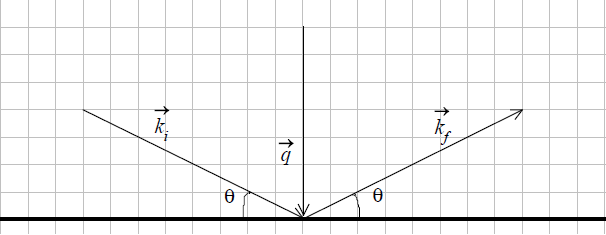
\includegraphics[width=0.7\textwidth]{billede3.png}
\caption{\label{Billede}}
\end{figure}

Når vi arbejder med guides, er vi ofte interesseret i den kritiske vinkel, hvilket er den størst mulige vinkel, hvorved vi kan få total refleksion mellem guide og neutron. Når vi har total refleksion, gælder det at længden af $\vec{k_i}$ er lig længden af $\vec{k_f}$, hvilket vi blot vil kalde for k:
\begin{align}
k_i=k_f=k
\end{align}
(Noter, at vi blot skriver længden af $\vec{k_i}$ og $\vec{k_f}$ som $k_i$ og $k_f$) \\
Når vi ved dette, kan vi ved hjælp af simpel trigonometri skrive længden af $\vec{q}$ som:
\begin{align} \label{eq:q1}
q=2k \cdot sin(\theta)
\end{align}
Hvor $\theta$ er vinklen som neutronen reflekterer med. Hvis vi gør brug af vores definition af $k$, får vi at ligning (\ref{eq:q1}) kan skrives som:
\begin{align} \label{eq:q2}
q=4\pi \cdot \frac{sin(\theta)}{\lambda}
\end{align}
Hvor $\lambda$ altså er bølgelængden for neutronen. Da vi har ved små vinkler at gøre, kan vi approksimere ligning (\ref{eq:q2})  ved $sin(\theta)≈\theta$. Vi får at:

\begin{align}
q≈4\pi \cdot \frac{\theta}{\lambda}
\end{align}

Som sagt er det ofte relevant at kigge på den kritiske vinkel, hvilket altså er den størst mulige vinkel, hvorved totalrelfleksion er mulig. Denne vinkel betegner vi som $\theta_c$. Når vi har totalrefleksion ved den kritiske vinkel, har vi en kritisk spredningsvektor, hvis længde vi betegner med $q_c$. For et givent materiale er $q_c$ konstant, og vi ser derfor, at den kritiske vinkel er en funktion af bølgelængden. Vi får at:

\begin{align}
q_c≈4\pi \cdot \frac{\theta_c(\lambda)}{\lambda}
\end{align}

Vi har, at værdien for den kritiske spredningsvektor for nikkel er $q_{c, Ni}=0.0217\text{Å} ^{-1}$ \cite{lefmann_arleth_kirkensgaard_lebech_thomsen}. Dette er en fast værdi for nikkel, og vi kan dermed let udregne den kritiske vinkel som funktion af neutronens bølgelængde som: 

\begin{align}
\frac{q_{c,Ni} \cdot \lambda}{4\pi}=\theta_c(\lambda)
\end{align}

Vi får hermed ved simpel indsætning, at neutroner med en bølgelængde på 1Å har en kritisk vinkel på omtrent $0.1^∘$, mens neutroner med bølgelængde på 10Å har en kritisk vinkel på omtrent $1^∘$, på et neutronspejl lavet af nikkel.
Man kan dog opnå en højere værdi af $q_c$ ved at lægge lag af andre materialer, mellem lagene af nikkel. Denne værdi af $q_c$ udregnes som:

\begin{align}
q_c=m \cdot q_{c,Ni}
\end{align}

Hvor m er den såkaldte m-værdi. Denne er altså en indikation på hvor stor en kvalitet spejlet har, i forhold til et rent Ni-spejl. m værdien for et spejl er ofte på et par stykker, men kan komme helt op på 7. \cite{lefmann_arleth_kirkensgaard_lebech_thomsen}

\subsubsection{Eliptiske guides}
Når vi samler en række neutronspejle i forlængelse af hinanden, kalder vi det for en neutronguide. De simpleste guides er selvsagt fuldstændig lige. Dette er dog ikke altid det mest hensigtsmæssige. Der kan være flere forskellige grunde til, at man vil have en enten kurvet eller eliptisk guide. Hvis neutronerne skal transportereres store afstande, kan det være en fordel at gøre guiden breddere, ved at gøre den enten eliptisk, eller delvis eliptisk i starten. Derved kommer der længere flyvetid mellem hvert sammenstød mellem neutronen og guiden, og færre neutroner går dermed tabt. Derudover kan der være en idé i, at få den prøve man skyder på, uden for synslinje af neutronkilden, således at man ikke får baggrundsstråling. Dette kan gøres ved enten at lave en kurvet guide, eller eventuelt lave et såkaldt 'kink'. Et kink består af et neutronspejl, der reflekterer neutronerne fra en guide til en anden, så man kan få en vinkel mellem sine to neutronguides. 
Det kan også være nødvendigt at samle guiden på visse steder. Dette kan eksempelvis være nødvendigt, hvis man vil indsætte en såkaldt chopper.

\subsubsection{Chopper}
En chopper er en roterende komponent, der kun lader neutroner passere i visse tidsintervaller. Den simpleste chopper er en 'disk chopper', som basalt set er en roterende disk, med et antal 'revner' eller huller nær kanten. Chopperen bliver sat til at rotere foran neutronstrålen, og neutronerne kan dermed kun passere chopperen, når chopperen er åben, dvs. når neutronen kan passere gennem hullet i chopperen. I det chopperen roterer, vil det kun til nogle tidspunkter være muligt for neutronerne at passere. Med en chopper kan man altså opdele neutronstrålen i midnre bider. Dette kan give en bedre kontrol over neutronerne, og dermed bedre resultater.

\subsubsection{Neutronkilder og moderator}
Neutroner kan genereres på flere forskellige måder. Ved ESS i Lund bliver neutronerne frembragt ved protonbombardament af en wolframkilde. Alle neutronerne skal helst have samme hastighed, og for at give dem dette gør man brug af en såkaldt moderator.

Vi har i introduktionen allerede beskrevet det her... Kan ikke finde noget om butterfly?
\cite{ess_folder}

\subsubsection{Neutron detektion}
Efter neutronerne har interergeret med prøven, skal de selvsagt detekteres, således at man kan 
For at måle kvaliteten af forsøgene, bruges forskellige slags monitors (også i simuleringer)





\subsection{Krav til guidesystemerne}
De forskellige guides der bliver bygget, skal bruges til forskellige eksperimenter, hvorfor deres specifikationer er forskellige. BIFROST som bearbejdes i dette projekt må koste op til 2.10 M€, hvilket selvfølgelig har betydning for vores optimeringsmuligheder. Prøven skal befinde sig 165m fra kilden, derfor skal guiden være 163m lang, da de første 2m skal være fri. Endvidere må guiden højst have et tværsnit på 0.1m på sit breddeste, for at mindske arealet, idet prisen ellers ville blive for høj pga. substrate, der i størstedelen af guiden er borcron og koster $14.000 \text{€}/m^2$. I de første 23.5m består substraten af aluminium, der koster $25.000 \text{€}/m^2$. Udover prisen som en begrænsende faktor, skal der indsættes choppers 0.5m og 23.5m inde i vores guide, det resulterer i, at guidens tværsnit skal sænkes på disse steder, så neutronerne kommer gennem chopperne. Det er vigtigt for eksperimentet, at neutronerne har den rette energi, derfor skal prøven være uden for synslinje fra kilden, da neutronerne med for høje energier ikke bliver reflekteret, men fortsætter gennem spejlet.

\subsection{Bedømmelse af guidesystemer}
Her snakker vi om hvordan vi bedømmer guidesystemerne, dvs. antal neutroner, divergens, brilliance transfer osv.

\subsection{Svagheder og fejlkilder ved MCstas}
Hvorfor er det godt og hvorfor er det skidt?



\section{Resultater}

\subsection{Vores guide(s)}
Plots of beskrivelse af vores guides



\section{Diskussion}

\subsection{Bedømmelse af vores guides}
Her snakker vi om styrker/svagheder ved vores systemer

\section{Konklusion}



%% Rapporten er slut! %% 
\newpage
%% Kilder %%

\bibliographystyle{plain}
\bibliography{sources} 

%% Kilder er slut! %% 
\newpage
%% Appendix %%

\appendix
\section{Appendix}
PDF, ESS Gymnasiehæfte

%% Appendix slut! %%

\end{document}

